
%%%%%%%%%%%%%%%%%%%%%%% file typeinst.tex %%%%%%%%%%%%%%%%%%%%%%%%%
%
% This is the LaTeX source for the instructions to authors using
% the LaTeX document class 'llncs.cls' for contributions to
% the Lecture Notes in Computer Sciences series.
% http://www.springer.com/lncs       Springer Heidelberg 2006/05/04
%
% It may be used as a template for your own input - copy it
% to a new file with a new name and use it as the basis
% for your article.
%
% NB: the document class 'llncs' has its own and detailed documentation, see
% ftp://ftp.springer.de/data/pubftp/pub/tex/latex/llncs/latex2e/llncsdoc.pdf
%
%%%%%%%%%%%%%%%%%%%%%%%%%%%%%%%%%%%%%%%%%%%%%%%%%%%%%%%%%%%%%%%%%%%


\documentclass[runningheads,a4paper]{llncs}

\usepackage{amssymb}
\setcounter{tocdepth}{3}
\usepackage{graphicx}

\usepackage{url}
\urldef{\mailsa}\path|{alfred.hofmann, ursula.barth, ingrid.haas, frank.holzwarth,|
\urldef{\mailsb}\path|anna.kramer, leonie.kunz, christine.reiss, nicole.sator,|
\urldef{\mailsc}\path|erika.siebert-cole, peter.strasser, lncs}@springer.com|    
\newcommand{\keywords}[1]{\par\addvspace\baselineskip
\noindent\keywordname\enspace\ignorespaces#1}

\begin{document}

\mainmatter  % start of an individual contribution

% first the title is needed
\title{Sistema de Recuperación de Información}

% a short form should be given in case it is too long for the running head
\titlerunning{Sistema de Recuperación de Información}

% the name(s) of the author(s) follow(s) next
%
% NB: Chinese authors should write their first names(s) in front of
% their surnames. This ensures that the names appear correctly in
% the running heads and the author index.
%
\author{Carlos Rafael Ortega Lezacano \and Eric Martín García \\ Grupo C511}
%
\authorrunning{Sistema de Recuperación de Información}
% (feature abused for this document to repeat the title also on left hand pages)

% the affiliations are given next; don't give your e-mail address
% unless you accept that it will be published
\institute{Universidad de la Habana}

%
% NB: a more complex sample for affiliations and the mapping to the
% corresponding authors can be found in the file "llncs.dem"
% (search for the string "\mainmatter" where a contribution starts).
% "llncs.dem" accompanies the document class "llncs.cls".
%

\toctitle{Sistema de Recuperación de Información}
\tocauthor{Authors' Instructions}
\maketitle

\section{Introducción}

Los sistemas de recuperación de información brindan un manejo efectivo de un conjunto considerable de datos, poder realizar consultas a un conjunto de documentos por parte de los usuarios es una característica fundamental en estos, hoy en día son de vital importancia para todos, a diario realizamos búsquedas en Google, ResearchGate entre otros sitios los cuales cuentan con un volumen de información considerable. 

La primera descripción de una computadora que buscaba información fue descrita por Holmstrom en 1948, detallando una mención temprana de la computadora Univac. Los sistemas automatizados de recuperación de información se introdujeron en la década de 1950. En la década de 1960, Gerard Salton en Cornell formó el primer gran grupo de investigación de recuperación de información. En la década de 1970, se había demostrado que varias técnicas de recuperación diferentes funcionaban bien en corpus de texto pequeños, como la colección Cranfield (varios miles de documentos). Los sistemas de recuperación a gran escala, como el sistema Lockheed Dialog, se empezaron a utilizar a principios de la década de 1970. 

En este escrito analizaremos la implementación realizada de un IRS, primeramente exponiendo los conceptos teóricos empleados para el diseño del sistema, las herramientas empleadas para el procesamiento de los corpus y por último como se realiza la evaluación del modelo. 

\section{Diseño del Sistema}

Un sistema de recuperación de información (IRS) se compone por el cuadruplo $<D,\ Q,\ F,\ R(q_j, d_j)>$, donde $D$ es un conjunto de representaciones de los documentos, $Q$ es un conjunto compuesto por representaciones lógicas de los pedidos que el usuario realiza al sistema, $F$ es un framework para modelar las representaciones y $R$ es una función de orden donde a cada consulta $q_j$ y un documento $d_j$ le asigna un valor acorde a la relevancia del documento para esa consulta. El proceso de interacción de un sistema con un usuario sigue el siguiente comportamiento: Primeramente el usuario realiza una consulta (un elemento de $Q$), esta pasa al motor de búsqueda, este es la componente más importante del sistema ya que en este se realizan las representaciones de los documentos\footnote{En nuestro caso es un IRS vectorial por tanto la representación interna se realiza mediante vectores cuyas componentes son pesos asociados a la entidad resultante del preprocesamiento}, además de representar la consulta en formato interno, el sistema dará como resultado una lista ordenada por relevancia de los documentos del corpus. Analizaremos a continuación el procesador de consultas, como se compone el motor de búsqueda y finalmente la salida del sistema. En nuestro caso el sistema va enfocado en la búsqueda de documentos, un documento tiene varias características, dos de las más comunes y útiles a la hora de realizar búsquedas es el título y el cuerpo del documento.

\subsection*{Motor de Búsqueda}

El motor de búsqueda contiene el modelo de recuperación de información, además en este se realiza el preprocesado de los documentos y su representación interna, también cada consulta se almacena en su forma interna para ser empleada en otras tareas. Además contiene la función de ranking la cual clasifica la relevancia de los documentos del corpus acorde a la consulta y el IRS.

\subsubsection{Preprocesamiento:} 

Para representar los documentos primeramente es necesario realizar un preprocesado, en nuestro sistema procedemos de forma simple empleando recursos del procesamiento de lenguaje natural. Las siguientes transformaciones son realizadas para cada documento del corpus:

\begin{enumerate}
	\item \textbf{Tokenizar el documento:} Primeramente es necesario crear la representación básica de un documento, la división en tokens, estos son unidades básicas, de esta forma podemos realizar procesamiento más avanzado sobre el texto, ya desde esta parte del procesamiento podemos llevar a minúscula todas las palabras, eliminar símbolos y signos de puntuación. También es posible convertir los números a texto, de esta forma no tendremos problemas a la hora de construir los diversos modelos. \\
	\item \textbf{Eliminación de \textit{stopwords}:} Las \textit{stopwords} como sabemos son palabras vacias de significado, las cuales pueden servir de nexo entre entidades o funcionan como modificadores. Si incluimos estas palabras en la representación del documento se afecta la efectividad del modelo debido a la alta frecuencia que poseen estas palabras en los textos. \\
	\item \textbf{Stemming:} Este método busca relacionar palabras con igual significado
	pero que difieren en cuanto a la escritura, por la aplicación de prefijos o
	sufijos, se encuentran en plural o singular entre otras diferencias, en este caso no usaremos lematización que es común que se emplee luego del stemming, con remover las partes correspondientes es suficiente para obtener buenos resultados.
\end{enumerate} 

Estas técnicas son las empleadas por el sistema para obtener un conjunto de textos formados por entidades con un significado y peso correcto para empezar a construir el modelo, pero antes de definir el modelo es necesario definir como serán estas entidades y que representación interna tendrán. Se eligió emplear los tokens como entidad del sistema, de esta forma se construye una colección con el siguiente formato:  \\

\noindent
{\it Representación del titulo y el cuerpo del documento preprocesado}
\begin{verbatim}
	    corpus: {
                   [id: n,
                   'title': Tokenize(doc_title),
                   'body': Tokenize(doc_body),
                   ],
                   ...
             }
\end{verbatim}
%
\noindent

\subsubsection{Vectorización:} De esta forma contamos con el identificador para cada documento del corpus, su titulo y cuerpo preprocesado. Pero todavia tenemos tokens los cuales no pueden ser la entrada para el modelo, es necesario realizar una vectorización
empleando TF-IDF. Para calcular los valores de frecuencia emplearemos el titulo y el cuerpo del documento juntos, sin realizar distinción, o sea el titulo podría ser una oración más del texto.

\paragraph*{TF-IDF:} Es una técnica para cuantificar una palabra en documentos, generalmente calculamos un peso para cada palabra que significa la importancia de la palabra en el documento y corpus. Este método es una técnica ampliamente utilizada en recuperación de información y minería de textos. Esta se representa por $w(t_i, d_j)$ donde $t_i$ es un término del documento $d_j$, en nuestro caso un los $t_j$ son tokens. \\

El TF-IDF se compone de dos conceptos fundamentales que se apoyan en el procesamiento de los documentos, el TF (Frecuencia de Termino) y el IDF (Frecuencia Inversa de Documento).

\paragraph*{TF:} Mide la frecuencia de una palabra en un documento. Esto depende en gran medida de la longitud del documento y de la generalidad de la palabra, por ejemplo, una palabra muy común como "casa" puede aparecer varias veces en un documento. Como los documentos pueden tener una longitud variable entonces contar simplemente las palabras podría dar prioridad a documentos de mayor tamaño, por eso es que se divide la cantidad de ocurrencias por el número total de palabra del documento $N(d_j)$. TF es individual para cada documento y palabra, por lo tanto, podemos formular TF de la siguiente manera:

\begin{equation}
	f_s(t_i, d_j) = \frac{C(t_i, d_j)}{N(d_j)}
\end{equation}

Donde $C(t_i, d_j)$ representará la cantidad de ocurrencias del termino en el documento. Recordemos que estamos vectorizando los documentos por tanto es necesario introducir el concepto de \textbf{vocabulario}, este es un conjunto formado por todas las palabras del corpus, o sea todas las palabras que hay en cada documento, de esta forma garantizamos que los vectores para cada documento tengan siempre las misma dimensión, donde cada componente tendrá el valor de frecuencia asociado para esa palabra, este estará en el intervalo $[0,1]$. Aunque empleando esta frecuencia es posible obtener resultados, todavía podemos mejorar los valores para el vector. Antes de definir IDF es necesario definir Frecuencia de Documento, ya que su inversa es IDF.

\paragraph*{DF:} Esto mide la importancia del documento en todo el conjunto de corpus, esto es muy similar a TF. La única diferencia es que TF es el contador de frecuencia para un término t en el documento d, donde DF es el recuento de apariciones del término $t_i$ en el conjunto de documentos $D$. En otras palabras, DF es el número de documentos en los que está presente la palabra. Consideramos una ocurrencia si el término consta en el documento al menos una vez, no necesitamos saber el número de veces que el término está presente. 

Como en el caso de TF también normalizamos dividiendo por el número total de documentos. Nuestro principal objetivo es conocer la informatividad de un término, para eso invertimos DF.

\paragraph*{IDF:} Es la inversa de la frecuencia del documento que mide la informatividad del término t. Cuando calculemos el IDF, será muy bajo para las palabras más frecuentes. Como es posible que el DF sea cero entonces es necesario realizar algunas modificaciones para no dividir entre 0, además si el corpus es grande podemos entonces obtener un valor que no sea de utilidad por lo tanto emplearemos para calcular el IDF.

\begin{equation}
	\overline{d}_s(t_i) = \log{\frac{|D|}{d_s(t_i) + 1}}
\end{equation}

Ahora combinemos ambas frecuencias, de esta forma tendremos una relación entre términos de mucha ocurrencia con respecto a aquellos que de baja frecuencia en los documentos.

\begin{equation}
	w(t_i, d_j) = f_s(t_i, d_j) \cdot \log{\frac{|D|}{d_s(t_i) + 1}}
\end{equation}

Hasta el momento se ha expuesto el concepto de TF-IDF para documentos pero ignorando si tienen titulo o no. Los textos que conforman el corpus del motor de búsqueda tienen diversas características y hemos elegido el titulo y el cuerpo para representar, por lo tanto debemos determinar cual de estos es más importante, o sea para dar un valor de relevancia a un documento que tiene mayor peso el título o el cuerpo, para ello definamos el parámetro $\alpha$ el cual define cuanto peso le damos al título a la hora de calcular la relevancia, de esta forma tendríamos que determinar los valores de TF-IDF tanto para el título como para el cuerpo, relacionando estos valores con $\alpha$ para obtener la frecuencia final para el término en el documento. Como los valores de TF-IDF para un término no toman en cuenta si este se encontraba en el titulo del documento o en el cuerpo, como se expreso anteriormente entonces definamos $w_t$ como el valor de TF-IDF para un término en el título y $w_b$ para cuando se encuentra en el cuerpo del documento. Finalmente obtenemos la expresión.

\begin{equation}
	w(t_i, d_j) = w_t(t_i, d_j) · \alpha + w_b(t_i, d_j) · (1 - \alpha), \qquad \alpha \in [0, 1]
\end{equation}

Podemos notar como el valor de $\alpha$ es un coeficiente asociado a las frecuencias de cada parte del documento, además un aspecto importante a tener en cuenta es lo siguiente: Si el termino $t_i$ aparece tanto en el título como en el cuerpo del documento entonces $w_t(t_i, d_j) = w_b(t_i, d_j)$, debido a que no se tomó en cuenta la posición a la hora de calcular los valores de frecuencia, por lo tanto el valor final sería: 

\begin{equation}
	w(t_i, d_j) = w_b(t_i, d_j)
\end{equation}

Ya tenemos el valor de frecuencia además de que empleamos el parámetro  $\alpha$ para definir la importancia que tiene el título o no al momento de determinar la relevancia, pasemos entonces a vectorizar los documentos. Para vectorizar el documento emplearemos un Bag of Words.

\paragraph*{Bag of Words:} Este consiste en tomar todas las palabras del corpus que constituyen el vocabulario ($V$) y formar una colección donde cada palabra tiene asociado un índice, de esta forma obtenemos un vector $\overrightarrow{d_j}$ de dimension $1 \times |V|$ asociado al documento $d_j$, donde en cada componente se encuentra el valor de TF-IDF asociado a la palabra.

De esta forma obtenemos para cada documento del corpus el vector $\overrightarrow{d_j}$, ahora pasemos a determinar como se procesa la consulta para obtener su vector correspondiente y dependiendo de este que función de ranking se empleó.

\subsection*{Consultas}

Como sabemos en el sistema existe un conjunto $Q$ que contiene las consultas realizadas por el usuario, una consulta $q$ no es más que una oración u entidad empleada para realizar la búsqueda. Para poder determinar cuales documentos son relevantes para esa consulta es necesario establecer un orden de los mismo acorde a la importancia por lo tanto debemos convertir la consulta a un vector empleando el mismo proceso que vimos en el motor de búsqueda.

Se usa el mismo vocabulario $V$ empleado para la representación del corpus, y se procese a crear el vector $\overrightarrow{q_i}$, en caso que existan palabras en $q_i$ que no se encuentran en el vocabulario serán ignoradas. 

El valor que tomarán las componentes no tiene necesariamente que ser calculo igual a como se realiza en el motor de búsqueda para representar el corpus, puede depender de la función de ranking o si usamos un modelo un poco más complejo. En nuestro caso tomamos dos representaciones vectoriales acorde a como se calculaba el ranking.

Para el caso de crear el vector usando TF-IDF se agrega un parámetro de suavizado $a$, el cual permite amortiguar la frecuencia, evitando que aparezcan grandes saltos de frecuencia o consecutivamente el mismo valor de frecuencia, por lo tanto obtendríamos:

\begin{equation}
	w_q(t_i, d_j) = \left( a + (1 - a)  · f_s(t_i, d_j) \right) \cdot \log{\frac{|D|}{d_s(t_i) + 1}}	
\end{equation}

\subsection*{Función de Ranking} 

Ahora es necesario relacionar la consulta con el corpus para determinar el valor de relevancia que tienen los documentos con respecto a la consulta realizada o sea debemos definir la función $R(q_i, d_j)$ para esto empleamos dos enfoques.

\paragraph{Puntuación Coincidente:} Una forma sencilla de calcular la similitud es emplear este enfoque primeramente representamos el vector de consulta $\overrightarrow{q_i}$ de forma binaria, asignando 1 para los términos que aparecen en la consulta, 0 en caso que no, luego para cada documento sumamos los valores de TF-IDF que tienen 1 en el vector consulta, de esta forma se obtiene el valor de similitud para realizar la ordenación.
Para realizar esta función solo es necesario hacer un producto escalar de los vectores

\begin{equation}
	R(q_i, d_j) = \overrightarrow{q_i} \cdot \overrightarrow{d_j} = \sum_{l = 0}^{|V|} w(t_l, d_j) \cdot w(t_l, q_i)
\end{equation}

De esta forma obtenemos mayores valores de relevancia para documentos que tengas valores de frecuencia alta para los términos que componen la consulta. Al representar el vector consulta solamente con 0 y 1 no aprovechamos la similitud que podría existir entre sus valores de frecuencia, o sea es posible que en la consulta podamos determinar que términos son más importantes que otros a la hora de realizar la búsqueda. 

\paragraph{Similitud del Coseno:} Primeramente colocaremos ahora el valor de TF-IDF asociado al término en la consulta y emplearemos el coseno del angulo comprendido entre los vectores consulta $\overrightarrow{q_i}$ y documento $\overrightarrow{d_j}$ para determinar la similitud, la función $R$ sería:

\begin{equation}
	R(q_i, d_j) = \frac{\overrightarrow{q_i} \cdot \overrightarrow{d_j}}{|\overrightarrow{q_i}| \cdot |\overrightarrow{d_j}|} = \frac{\sum_{l = 0}^{|V|} w(t_l, d_j) \cdot w(t_l, q_i)}{\sqrt{\sum_{l = 0}^{|V|} w^2(t_l, q_i)} \cdot \sqrt{\sum_{l = 0}^{|V|} w^2(t_l, d_j)}}
\end{equation}

Podemos apreciar como se busca establecer una relación entre los valores de frecuencia de la consulta y el documento de esta forma analizamos aquellos términos de la consulta que son más importantes y buscamos similitud con respecto al corpus.

\paragraph{Output del Sistema:} Una vez que tenemos la función de ranking pasamos a obtener los valores correspondientes para la consulta, ordenamos de forma descendente aquellos que son distintos de 0. Suministrando el titulo del documento y el valor obtenido.

\subsection*{Retroalimentación de Relevancia}

La retroalimentación de relevancia es una característica de algunos sistemas de recuperación de información . La idea detrás de la retroalimentación de relevancia es tomar los resultados que se devuelven inicialmente de una consulta determinada, recopilar la retroalimentación de los usuarios y utilizar información sobre si esos resultados son relevantes o no para realizar una nueva consulta. Podemos distinguir de manera útil entre tres tipos de retroalimentación: retroalimentación explícita, retroalimentación implícita y retroalimentación ciega o "pseudo".

Debido a que emplear el TF-IDF no siempre resulta en una representación confiable debido a que cuando representamos los vectores perdemos el significado semántico además de las relaciones entre los términos, por ello decidimos incluir un algoritmo de retroalimentación explícito en nuestro caso, con el objetivo de suministrar al usuario una manera de mejorar el vector consulta, así podemos resolver problemas de ambigüedad entre otros para esto elegimos el algoritmo de Rocchio el cual es abordado en \cite{rocchio}.

\subsubsection*{Algoritmo de Rocchio:} Un algortimo simple y muy conocido para la retroalimentación en los sistemas de recuperación de información es el algoritmo de Rocchio, el cual era empleado en los IRS que surgieron del Sistema de Recuperación de Información SMART, desarrollado en 1960-1964. El enfoque de retroalimentación de Rocchio se desarrolló utilizando el Modelo de Espacio Vectorial que empleaba SMART. El algoritmo se basa en la suposición de que la mayoría de los usuarios tienen una concepción general de qué documentos deben indicarse como relevantes o no relevantes para la consulta que realizan. Por lo tanto, la consulta de búsqueda del usuario se revisa para incluir un porcentaje arbitrario de documentos relevantes y no relevantes como un medio para aumentar la precisión del motor de búsqueda.

El algoritmo de rocchio busca realizar una mejora a la consulta que deseamos, podemos ver como consulta $\overrightarrow{q_i}$ realiza una bipartición del conjunto $D$ en dos conjunto $D_R$ donde se encuentran aquellos documentos cuya relevancia es distinta de 0 y $D - D_R$ serán aquellos que no son relevantes. Ahora debemos encontrar una consulta optima a partir de $\overrightarrow{q_i}$ para la cual se maximice la similitud con el conjunto de documentos relevantes $D_R$ implicando un valor mínimo de similitud para el conjunto de textos no relevantes:

\begin{equation}
	\overrightarrow{{q_i}}_{opt} = \verb*|argmax|_{\overrightarrow{q_i}} \left[ R(\overrightarrow{q_i}, D_R) - R(\overrightarrow{q_i}, D - D_R) \right] 
\end{equation}

Podemos emplear como $R$ la similitud del coseno vista anteriormente o también el centroide del conjunto de documentos seleccionado, este último resulta más útil que ya que necesitamos reducir la similitud acorde a un subconjunto de $D$, aplicando el centroide y sustituyendo se obtiene:

\begin{equation}
	\overrightarrow{{q_i}}_{opt} = \frac{1}{|D_R|} \sum_{\overrightarrow{d_j} \in D_R} \overrightarrow{d_j} - \frac{1}{|D - D_R|} \sum_{\overrightarrow{d_j} \notin D_R} \overrightarrow{d_j} 
\end{equation}

Este enfoque no es muy utilizado frecuentemente debido a que el conjunto $D$ puede ser muy grande por lo tanto determinar el centroide sobre una bipartición para optimizar la consulta no resultará muy eficiente. Por eso se emplean 3 parámetros $\alpha, \beta $ y $\gamma$  para definir peso asociado a la consulta original, el conjunto de documentos relevantes y el de no relevantes, de esta forma podemos seleccionar subconjuntos. La expresión matemática final será:

\begin{equation}
	\overrightarrow{q_m} = \alpha · \overrightarrow{q_0} + \beta \frac{1}{|D_R|} \sum_{\overrightarrow{d_j} \in D_R} \overrightarrow{d_j} - \gamma \frac{1}{|D - D_R|} \sum_{\overrightarrow{d_j} \notin D_R} \overrightarrow{d_j}
\end{equation}

Donde $\overrightarrow{q_0}$ es el vector de la consulta que se desea optimizar, $D_R$ es el conjunto formado por los documentos relevantes, los parámetros funcionan como valores de confianza a la hora de operar con cada miembro de la expresión, por ejemplo si quisiéramos tener muchos documentos en ambas categorías entonces deberíamos dar valores mayores a $\beta$ y $\gamma$. Al aplicar esta expresión la consulta original se acerca más hacia el centroide de documentos relevantes y se aleja de los no relevantes, está nueva consulta será ahora la empleada por el IRS. Los valores negativos en el nuevo vector se asumen como 0, debido a que solamente son validos los valores para el primer cuadrante. Como hemos dicho esto mejora la precisión y el recall del sistema, principalmente en la práctica se ha demostrado como el recall es el más beneficiado ayudando a optimizar la búsqueda. Un aspecto importante es como la interacción con el usuario determina que tan buen valor de recall obtenemos, el tiempo que tomen en revisar los resultados, evaluarlos y determinar si satisface lo deseado es fundamental. En la práctica es común usar $\alpha = 1, \beta = 0.75$ y $\gamma = 0.15$, como se aprecia se busca mantener el sentido de la consulta original y obtener la mayor cantidad de documentos relevantes.

\section{Sobre la implementación} % aqui link a github

La implementación del sistema se realizó en \verb*|Python|, ya que cuenta con muchas herramientas para el procesamiento de texto, la representación de vectores de forma optima y al ser tan empleado para realizar trabajos con IRS se cuenta con una extensa documentación.

El objeto que representa el IRS es \verb*|IrSystem|, el cual contiene las implementaciones de los temas abordados en la sección anterior. Para crear una instancia se emplea el valor de $\alpha$ para definir el peso que se le da al título de los documentos, y la dirección del dataset que será empleado, el cual contiene el corpus. Si nuestro corpus no contiene textos con título solamente tendremos que hacer $\alpha = 0$, para que no se tome en cuenta el peso del título.

\noindent
%
\begin{verbatim}
	class IrSystem:	   
	   def __init__(self, alpha, dataset):
	      ...
	      
	   def preprocess(self, data):
	     ...	     
	   ...
\end{verbatim}
%
\noindent

Para realizar el preprocesado empleamos \textbf{nltk}, que es una poderosa herramienta en el procesamiento de lenguaje natural. Para retirar las stopwords se empleo \verb*|nltk.corpus.stopwords| que brinda una colección extensa de palabras en ingles. Para el proceso de stemming se usó \verb*|nltk.stem.PorterStemmer|, el PorterStemmer retira sufijos y prefijos de las palabras dejando solamente la raíz, es tal vez uno de los más empleados. Adicionalmente para tokenizar el texto preprocesado se empleo \verb*|nltk.tokenize.word_tokenize|.

Para el proceso de vectorización se emplean matrices esparcidas las cuales permiten representar vectores con 0 en muchas de sus componentes, para esto empleamos \verb*|scipy.sparse|. Para construir estos vectores primero se termino el vocabulario y luego se paso a implementar los cálculos de frecuencia. Para realizar calculos más comodos y poder manejar el conteo se empleo \verb*|numpy| y \verb*|collection.Counter|, de esta forma se crearon las funciones para calcular los pesos.

El algoritmo de ranking emplea la similitud del coseno para determinar el orden en que serán dispuestos los documentos, usando la función \verb*|search| se realiza todo el proceso:

\noindent
%
\begin{verbatim}
	def search(self, query, query_id = False, k = -1, 
	                               show_output = True, preview = 500):
	    ...
	    preprocessed_query = self.__preprocess(query)
	    ...
	    
	    tokens = word_tokenize(str(preprocessed_query))
	    
	    d_cosines = []
	    
	    query_vector = self.__gen_query_vector(tokens)
	    
	    for d in self.tf_idf:
	    d_cosines.append(IrSystem.__cosine_sim(d, query_vector))	    
	    out = [(id, d_cosines[id].max()) for id in np.array(d_cosines).
	                argsort()[-k:][::-1] if d_cosines[id].max() > 0.0]	    
	    self.searched[query_id] = (query, out)
	    ...
\end{verbatim}
%
\noindent

Esta función es la más importante ya que realiza el ranking de documentos según la relevancia, como se observa primero realiza el preprocesamiento de la consulta y luego la tokeniza para poder formar el vector, empleando el vector emplea los vectores internos resultantes del proceso de interpretación de los documentos para calcular la similitud y obtener la salida del sistema, las consultas con sus respectivos resultados son almacenadas para poder aplicar la retroalimentación mediante el algoritmo de Rocchio.

% Falta: Explicacion codigo rocchio 

Para la evaluacion del sistema se implementaron las tres medidas de evaluación, precision, recobrado y f1-score. Estas estan pensadas para poder evaluar una consulta de forma individual, para ello se define una función que determina los documentos relevantes recuperados para la consulta y de esa forma se calculan las tres medidas fundamentales \verb*|get_recall|, \verb*|get_precision| y \verb*|f1_score|. Para determinar los resultados globales, o sea tomando en cuenta todas las consultas se emplea \verb*|numpy| para el promedio de los valores.
Para visualizar la relación entre la precisión y el recobrado se cuenta con la función \verb*|plot_results| que muestra la gráfica P/R correspondiente, ya sea para una consulta en particular o de forma global.  

\section{Evaluación del Sistema}

Para poder realizar la evaluación del sistema es necesario contar con colecciones de prueba, nuestro sistema emplea dos colecciones \textit{Cranfield} y \textit{MED} que es un corpus médico. Definiremos cuatro conjuntos fundamentales para definir las medidas de evaluación. 

\begin{enumerate}
	\item[] \textbf{RR:} Conjunto de Documentos recuperados relevantes
	\item[] \textbf{RI:} Conjunto de Documentos recuperados irrelevantes
	\item[] \textbf{NR:} Conjunto de Documentos no recuperados relevantes
	\item[] \textbf{NI:} Conjunto de Documentos no recuperados irrelevantes
\end{enumerate}

Los documentos recuperados irrelevantes pueden ser considerados como falsos
positivos, pues se recuperaron pero no eran interesantes para el usuario. De
manera análoga, los documentos no recuperados relevantes son los falsos
negativos. Empleando estos conjuntos definimos las siguientes medidas de evaluación:

\subsubsection*{Precisión:} Razón de los documentos relevantes que son recuperados

\begin{equation}
	P = \frac{|RR|}{|RR \cup RI|}
\end{equation}

En el campo de la recuperación de información no solo interesa qué tan precisa es la
respuesta, también que incluya a la mayor cantidad posible de documentos
relevantes, por lo tanto la medida de precisión por sí sola no es suficiente en
el caso de un modelo de recuperación de información.

\subsubsection*{Recobrado:} Razón entre los documentos relevantes que fueron recuperados.

\begin{equation}
	R = \frac{|RR|}{|RR \cup NR|}
\end{equation}

Este es fundamental en los procesos de
recuperación de información. Al contrario de la precisión el recobrado
aumenta a medida que incorporamos más documentos a la respuesta, pues es
cada vez más probable que los elementos del conjunto de documentos relevantes
estén contenidos en nuestra respuesta.

Es importante notar que las dos metidas ($P$ y $R$) se compensan, la precisión tiende a decrecer cuando la cantidad
de documentos recuperados aumenta y siempre es posible obtener $R = 1$, si recuperamos todos los documentos para la consulta, pero en este caso obtendríamos una precisión baja. La solución ideal plantea un alto valor de recobrado tolerando la menor cantidad posible de falsos positivos, es decir, de documentos recuperados irrelevantes.

\subsubsection*{Medida $F_1$:} Medida que armoniza Precisión y Recobrado teniéndolos en cuanta a ambos.

\begin{equation}
	F_1 = \frac{2 PR}{P + R}
\end{equation}

La medida $F_1$ toma un valor alto cuando Precisión y Recobrado son altos, por lo que $F_1$ puede verse como el intento de encontrar la mejor relación entre $P$ y $R$, donde ambos tienen igual importancia ($\beta = 1$)

\section{Resultados Obtenidos}

Empleando los datasets para evaluar el sistema empleando las medidas expuestas obtenemos una serie de resultados que permiten saber que tan eficiente es el IRS implementado. Para ello se emplea un archivo que contiene los valores de relevancia esperados. 

El proceso de evaluación del sistema permite primeramente seleccionar el dataset a usar para las pruebas, luego se realiza una corrida del sistema, recibiendo como entrada todas las consultas de prueba, así se obtienen para cada una los valores de medidas junto a los de documentos relevantes, después de esto contamos con un IRS que ha procesado y almacenado todas las consultas de prueba para el dataset, podemos en este punto realizar 3 acciones:

\begin{enumerate}
	\item Realizar una nueva consulta, esto permite añadir nuevas consultas para continuar testeando el sistema
	\item Calcular las medidas por consulta y global además de generar el grafico P/R 
	\item Mejorar la consulta mediante retroalimentacion de Rocchio
\end{enumerate}

La primera acción podemos emplearla para ver que textos fueron seleccionados y en que orden para una consulta, sea de prueba o una nueva que decidamos formular. La segunda operación comprueba las medidas del sistema, por ejemplo, si tenemos la primera consulta del dataset Cranfield: \\

\begin{verbatim}
	what similarity laws must be obeyed when constructing aeroelastic 
	models of heated high speed aircraft
\end{verbatim}

Para esta consulta se determinaron los valores de precision, recobrado y f1-score obteniéndose:

\begin{figure}
	\centering
	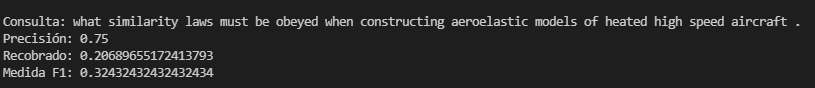
\includegraphics[height=1.3cm]{imgs/eval_query1_cran.png}
	\caption{Medidas para la primera consulta del Cranfield}
	\label{fig:cran1}
\end{figure}

Se observa la relación existente entre precision y recobrado, para una mejor representación se emplea el grafico P/R:

\begin{figure}
	\centering
	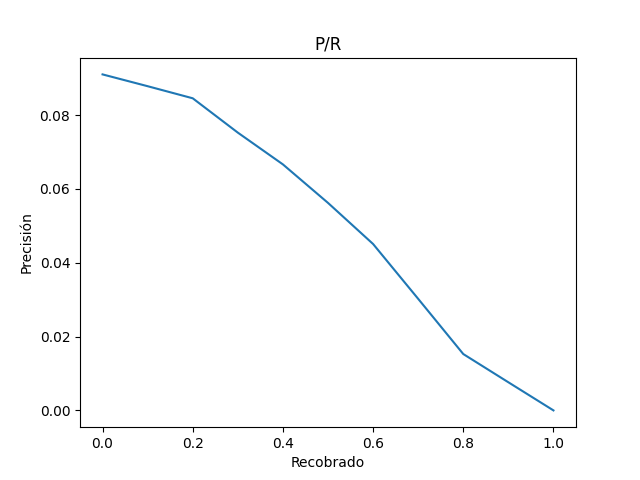
\includegraphics[height=6.3cm]{imgs/pr_query1_cran.png}
	\caption{Gráfica P/R para la primera consulta del Cranfield}
	\label{fig:cran1img}
\end{figure}

Ahora determinemos de forma general las medidas para todo el dataset de Cranfield, de esta forma sabremos el promedio de documentos relevantes recuperados (Fig. \ref{fig:cran1gen}).

\begin{figure}
	\centering
	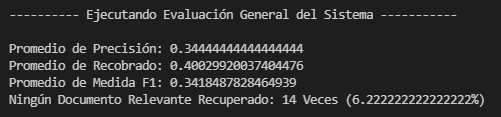
\includegraphics[height=2.3cm]{imgs/eval_general_cran.png}
	\caption{Medidas Generales para el Dataset de Cranfield}
	\label{fig:cran1gen}
\end{figure}

Estos resultados son aceptables tomando en cuenta que empleamos un modelo vectorial empleando TF-IDF con algunas modificaciones, entre algunas características extras se implementó un \textbf{query expansion} empleando WordNet que es un tesauro suministrado por NLTK, para cada termino de la consulta añadíamos sus sinónimos lematizados, al realizar las pruebas al sistema se redujo los valores de precisión y recobrado al obtener documentos que si bien podrían estar relacionados o vinculados al tema no eran considerados relevantes. Debido a eso se decidió que esta característica fuera empleada a la hora de realizar nuevas consultas por el usuario.

Ahora mostraremos los resultados para el dataset MED, el cual contiene textos sobres temas médicos, primeramente analizaremos los resultados para la consulta de prueba 27 y luego de forma general (los datos del dataset pueden ser encontrados en el código del sistema en \verb*|/dataset/MED|). La consulta 27 es la siguientes:

\begin{verbatim}
	interested in the parasitic diseases.  filaria parasites found 
	in primates, the insect vectors of filaria, the related diptera, 
	i. e.,culicoides, mosquitos, etc. that may serve as vectors of 
	this\ninfection-disease; also the life cycles and transmission of 
	the filaria.parasites and ecology of the taiwan monkey,macaca with
	cyclopis emphasis on the filarial parasite, macacanema formosana.
\end{verbatim}

Esta consulta fue seleccionada al ser extensa ademas que presenta abreviaturas, signos de puntuación dispuestos de forma excesiva y palabras mal colocadas, de esta forma podemos comprobar que tan bien recupera información asociada a esta. Los valores de medidas para esta son (Fig. \ref{fig:med1}) :

\begin{figure}
	\centering
	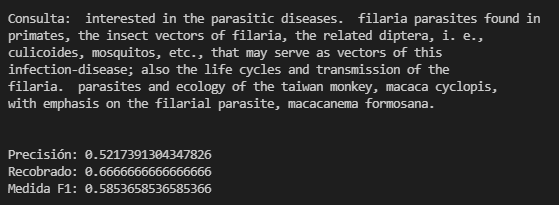
\includegraphics[height=3.3cm]{imgs/eval_query27_med.png}
	\caption{Medidas para la consulta 27 de MED}
	\label{fig:med1}
\end{figure}

Y su gráfico P/R es el siguiente (Fig. 5):

\begin{figure}
	\centering
	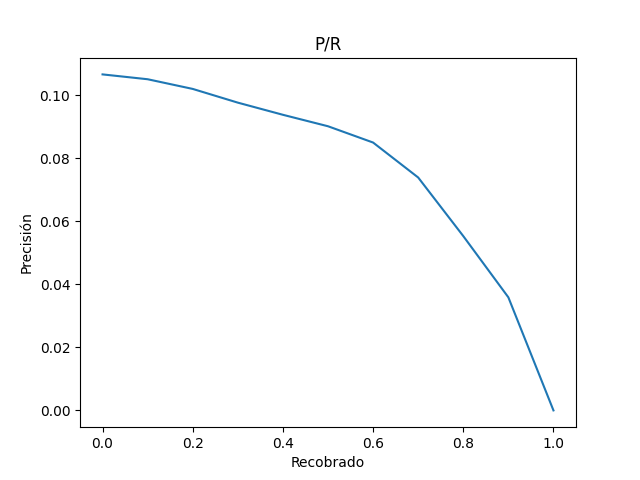
\includegraphics[height=6.3cm]{imgs/pr_query27_med.png}
	\caption{Gráfico P/R para la consulta 27 de MED}
	\label{fig:med1pr}
\end{figure}

Finalmente los valores de forma general para el dataset (Fig .6). 

\begin{figure}
	\centering
	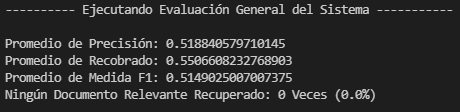
\includegraphics[height=2.3cm]{imgs/eval_general_med.png}
	\caption{Medidas Generales para el Dataset MED}
	\label{fig:med1gen}
\end{figure}

Estos resultados aunque sean mejor que para Cranfield, hay que tomar en cuenta la dimensión del dataset, en este caso el número de consultas y de documentos no es tan grande como el de Cranfield por lo tanto a la hora de la representación es posible que se tomen características más particulares de los documentos que conforman el corpus. 

% Falta como Rocchio mejora los valores

\section{Recomendaciones}

Al analizar los resultados obtenidos y las herramientas empleadas podemos plantear algunas modificaciones y proponer el uso de otros modelos para ver el comportamiento de los resultados.

La representación vectorial que se posee empleando Bag of Words no toma en cuenta ni la posición, ni las relaciones entre los términos, podría realizarse un enfoque empleando modelos de Semántica Latente para agregar cierto grado de interpretación a las consultas realizadas. Adicionalmente también podríamos agregar elementos de 
similitud semántica para una mejor expansión de las consultas realizadas por el usuario.

Agregar un modelo basado en entrenamiento, tales como Regresión Logística, Arboles de Decisión o Redes Neuronales puede ayudar construir una representación más expresiva del corpus y de esta forma podríamos obtener mejores resultados. Para evaluar estos modelos debemos dividir el dataset en dos conjuntos uno para entrenamiento y el otro para las pruebas al sistema.

Por último podría emplearse términos más expresivos, el sistema emplea palabras para construir los modelos, si en lugar de palabras empleáramos n-grams o subsecuencias máximas contaríamos con entidades más completas aunque esto conllevaría a que tenga que ser modificada la representación interna, debido a que puede aumentar considerablemente la dimensión de los vectores.

\begin{thebibliography}{4}

\bibitem{confs} C. Fleitas. Sistemas de Información, Departamento de Programación, Facultad de Matemática y Computación, Universidad de la Habana, 2021

\bibitem{rocchio} J.J. Rocchio. Document Retrieval Systems–Optimization and Evaluation.
PhD thesis, Harvard Computational Laboratory, Cambridge, MA, 1966.

\bibitem{lectures} H. Yannakoudakis. Lecture 7: Relevance Feedback and Query
Expansion Information Retrieval Computer Science Tripos Part II, Natural Language and Information Processing (NLIP) Group. University of Cambridge, 2018 

\bibitem{tds} \url{https://towardsdatascience.com/} : TF-IDF in Python

\bibitem{nltk} \url{http://www.nltk.org/} : NLTK API

\end{thebibliography}

\end{document}
